\documentclass{article}
% Chinese
% \documentclass[UTF8, nofonts, mathptmx, 12pt, onecolumn]{article}
% \usepackage{xeCJK}
% \setCJKmainfont{SimSun}
\usepackage{amsmath}
\usepackage{amsfonts}
\usepackage{amssymb}
\usepackage{wasysym}
% \usepackage{ctex}
\usepackage{graphicx}
\usepackage{float}
\usepackage{geometry}
\geometry{a4paper,scale=0.8}
\usepackage{caption}
\usepackage{subcaption}
% \newcommand{\oiint}{\mathop{{\int\!\!\!\!\!\int}\mkern-21mu \bigcirc} {}}
\newcommand*{\dif}{\mathop{}\!\mathrm{d}}
\newcommand*{\md}{\mathop{}\!\mathrm{d}}
\newcommand*{\me}{\mathrm{e}}

\usepackage{parskip}
\setlength{\parindent}{0cm}

\usepackage{bm}
\let\Oldmathbf\mathbf
\renewcommand{\mathbf}[1]{\boldsymbol{\Oldmathbf{#1}}}
\let\eqnarray\align

\renewcommand*{\arraystretch}{2}
\usepackage{units}
\renewcommand{\frac}{\nicefrac}

\usepackage{cellspace}
\setlength{\cellspacetoplimit}{5pt}
\setlength{\cellspacebottomlimit}{5pt}
\usepackage{siunitx}

\author{Xiping Hu}
\usepackage{authblk}
\author{Xiping Hu}
\affil{https://hxp.plus/}
\title{Homework for Chapter 8}

\begin{document}
\maketitle

\begin{figure}[H]
  \centering
  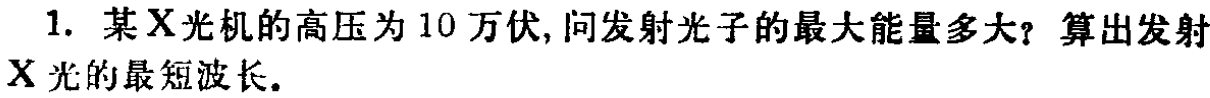
\includegraphics[width=\linewidth]{figures/Problem1}
  \label{fig:}
\end{figure}

\begin{equation*}
  \begin{aligned}
    E = 10 \times 10^5 \si{eV}
  \end{aligned}
  \quad\quad 
  \begin{aligned}
    \lambda = \dfrac{E}{h} = 0.124 \si{\angstrom}
  \end{aligned}
\end{equation*}

\begin{figure}[H]
  \centering
  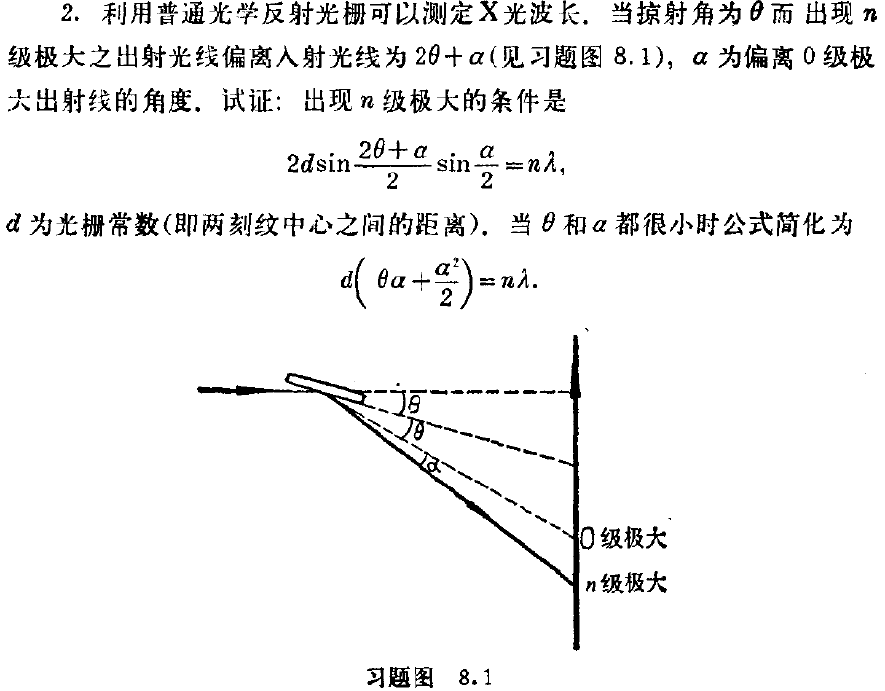
\includegraphics[width=\linewidth]{figures/Problem2}
  \label{fig:}
\end{figure}

\begin{figure}[H]
  \centering
  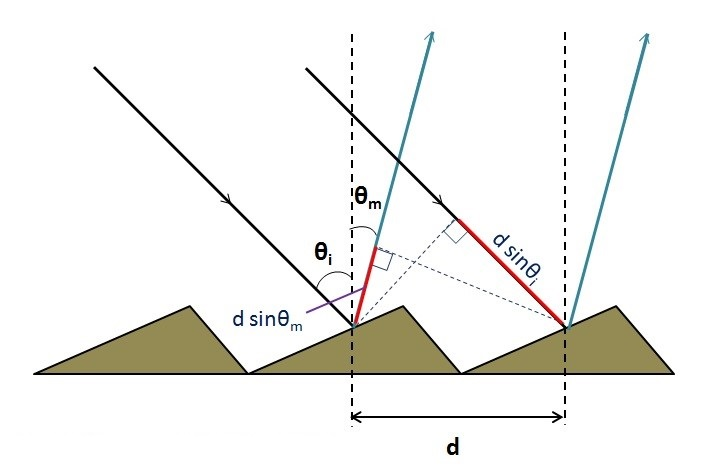
\includegraphics[width=0.7\linewidth]{figures/Problem22}
  \label{fig:}
\end{figure}

\begin{equation*}
  \begin{aligned}
    n \lambda = d \left[ \sin \left( \dfrac{\pi}{2} - \theta  \right) - \sin \left( \dfrac{\pi}{2} - \theta - \alpha \right) \right] = 2 d \sin \dfrac{2 \theta + \alpha}{2} \sin \dfrac{\alpha}{2}  
  \end{aligned}
\end{equation*}

In the case of $\theta \approx 0$ and $\alpha \approx 0$

\begin{equation*}
  \begin{aligned}
    n \lambda = 2 d \cdot \dfrac{2 \theta + \alpha}{2}  \cdot \dfrac{\alpha}{2} = d \left( \theta \alpha + \dfrac{\alpha^2}{2}  \right)
  \end{aligned}
\end{equation*}

\begin{figure}[H]
  \centering
  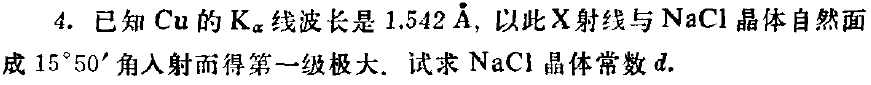
\includegraphics[width=\linewidth]{figures/Problem4}
  \label{fig:}
\end{figure}

\begin{equation*}
  \begin{aligned}
    d = \dfrac{\lambda}{2 d \sin \theta} = 2.825 \si{\angstrom} 
  \end{aligned}
\end{equation*}

\begin{figure}[H]
  \centering
  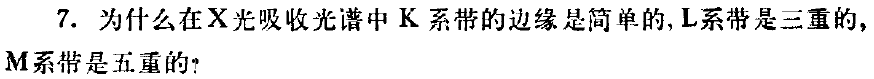
\includegraphics[width=\linewidth]{figures/Problem7}
  \label{fig:}
\end{figure}

In an X-rays tube an electron emitted from the cathode strikes the target with a tremendous velocity so that it penetrates well inside the atom of the target. If it ejects an electron from the K-shell of the atom, a vacancy is created in the K-shell. Immidiately an electron from one of the outer shells, say L-shell jumps to the K-shell, emitting an X-ray photon of energy equal to the energy difference between the two shells. And the maximum of energy an X-ray photon may have is equal to the energy of the ejected electron.

When $n=1$, the electron may has only one energy states: ${}^2S_{1/2}$. And $n=2$ has three energy states: ${}^2S_{1/2}$, ${}^2P_{1/2}$, ${}^2P_{3/2}$. $n=3$ has five energy states: ${}^2S_{1/2}$, ${}^2P_{1/2}$, ${}^2D_{3/2}$, ${}^2D_{5/2}$.

\end{document}